





\documentclass[11pt,a4paper]{scrartcl}
\typearea{12}
\usepackage{graphicx}
\usepackage{amsmath}
\usepackage{listings}
\usepackage{color}
\usepackage{tikz}
\usepackage{booktabs}
\usetikzlibrary{decorations.markings}
\lstset{language=C}
\usepackage{fancyhdr}
\pagestyle{fancy}
\begin{document}




\section*{Worksheet 8 - copied from Martha Lewis}

\subsection*{Q1: Gridworld and Value Iteration}

Consider the gridworld in Figure~\ref{fig:gridworld}.

\begin{figure}[h]
  \begin{center}
    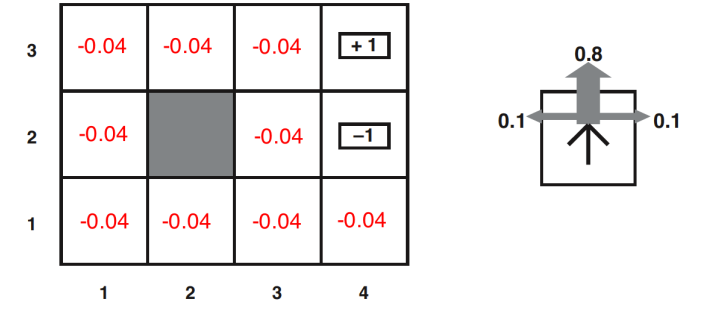
\includegraphics[width=8cm]{gridworld.png}
  \end{center}
  \caption{A gridworld! \label{fig:gridworld}}
  \end{figure}

(a) Do we need to wait until the algorithm has converged until we know the utility of each state, or are there some states whose utility we already know?

(b) Suppose we initialise the utility of every state to 0, and then perform one iteration of the value iteration algorithm. What is the utility of each state?

\subsection*{Q2: 3x3 Gridworld Policy}

Consider the 3x3 gridworld shown in Table~\ref{tab:gridworld}.

\begin{table}[h]
    \centering
    \begin{tabular}{ccc}
        \toprule
        r & -1 & 10 \\
        -1 & -1 & -1 \\
        -1 & -1 & -1 \\
        \bottomrule
    \end{tabular}
    \caption{3x3 Gridworld}
    \label{tab:gridworld}
\end{table}

The transition model is as follows: 80\% of the time the agent moves in the intended direction; the remaining 20\% of the time, it moves perpendicularly (10\% left, 10\% right). Given different values of $r$, determine the optimal policy using discounted rewards with $\gamma = 0.99$.

(a) $r = -3$

(b) $r = +3$

\subsection*{Q3: Bridge Crossing Problem}

Figure~\ref{fig:bridge} shows a narrow bridge gridworld where a robot must cross safely.


\begin{figure}[h]
  \begin{center}
    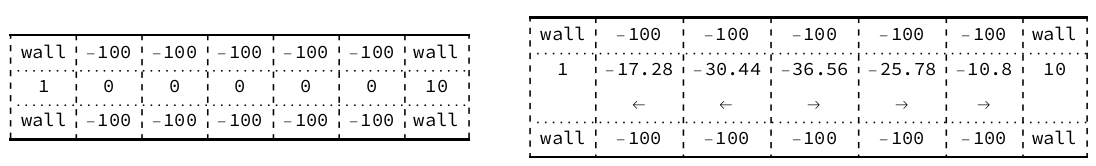
\includegraphics[width=15cm]{bridge.png}
  \end{center}
    \caption{Bridge crossing(a) rewards for the bridge-crossing problem in gridworld. (b) utilities after 5 iterations,
and the corresponding optimal policy}
    \label{fig:bridge}
\end{figure}

(a) Using a discount value of 0.9, calculate the utility of each non-terminal grid square after one and two moves.

(b) The optimal policy in Figure~\ref{fig:bridge} fails to cross the bridge. What is the effect of decreasing the discount value?

(c) What is the effect of increasing the utility of the goal? Choose a new value so that the optimal policy is to cross the bridge, and show the utility of each grid square after three iterations.

\end{document}
